\chapter{Un \textit{wearable device} pour la reconnaissance des sols}
\label{chap:4}

\section{Introduction}

Au cours des dernières années, les grands fabricants de matériel électronique tels que \textit{Garmin}, \textit{Apple}, \textit{Samsung} ou encore \textit{Fitbit} ont contribué à populariser les \textit{wearable devices} pour le grand public. En effet, selon le rapport réalisé par \cite{Nielsen2014}, 70\% des consommateurs interrogés connaissent cette technologie et 15\% d'entre eux se servent d'un \textit{wearable device} dans leur vie de tous les jours en plus de leur téléphone intelligent. Ces dispositifs ont permis l'exploitation de nouveaux types de capteurs, en comparaison de ceux qui étaient déjà présents dans les téléphones (\textit{p. ex.} les capteurs cardiaques) et ils ont permis d'accélérer l'adoption de technologies comme le \acs{BLE} \citep{Taplett}. En ce sens et puisqu'ils représentent un moyen pratique et portable pour enregistrer des données physiologiques,  les \textit{wearable devices} ont été rapidement et massivement adoptés, principalement pour assurer le suivi des activités sportives \citep{NPDGroup2015}. Il est donc devenu possible, pour leurs utilisateurs, de récolter une quantité considérable de données dans le but de produire des analyses statistiques et ainsi surveiller les évolutions dans la réalisation d'activités quotidiennes, qu'elles soient sportives ou non. Néanmoins, avec les avancements en matière d'apprentissage machine, il est possible d'affirmer que les applications développées spécifiquement pour les \textit{wearables devices} peuvent être améliorées pour devenir plus ubiquitaires.

L'objectif de ce chapitre est donc d'introduire un nouveau cas d'utilisation d'un wearable device où la réponse à la question suivante : \textit{« Est-il possible de reconnaître les types de sols à l'aide de données inertielles produites par la démarche humaine avec un wearable device\textemdash quel que soit l'endroit où il est porté ? »} est le principal sujet discuté dans deux publications respectivement présentées aux conférences \textit{IEEE 14th International Conference on Ubiquitous Intelligence and Computing (UIC)} qui s'est déroulée en août 2017 à San Francisco aux États-Unis \citep{Thullier2017a} et \textit{IEEE 15th International Conference on Ubiquitous Intelligence and Computing (UIC)} qui s'est déroulée en octobre 2018 à Guangzhou en Chine \citep{Thullier2018}.

Pour se faire, ce chapitre commence par présenter un état de l'art des recherches menées au sujet de la reconnaissance des sols par le biais de données inertielles. Ensuite, après avoir présenté la solution proposée ainsi que les expérimentations réalisées, ce chapitre va analyser et discuter les résultats obtenus. Finalement, la dernière partie dresse une conclusion de ce premier travail.

\section{État de l'art}
\label{sec:t1-related-work}

L'idée de reconnaître des types de sols par le biais de données produites par une centrale inertielle provient du domaine de la robotique. En effet, \cite{Vail2004} ont tout d'abord expérimenté la détection de surface grâce à des données inertielles produites par un robot quadrupède. Pour réaliser l'apprentissage, les auteurs ont opté pour un algorithme dont le modèle est un arbre de décision ($C4.5$), car ils estiment qu'il s'agit d'un algorithme suffisamment rapide et facile à représenter et à implémenter. Pour quantifier la précision de leur modèle d'apprentissage, \citeauthor{Vail2004} ont utilisé la technique de la validation croisée en 10-plis \citep{Kohavi1995}, ce qui leur a permis d'obtenir un taux de reconnaissance global de 84.9\% (ciment: 91\%; tapis: 81.2\%; champs: 81.2\%). Par la suite, \cite{Kertesz2016} ont également présenté une méthode permettant de reconnaître des sols avec un accéléromètre embarqué sur un robot quadrupède. Ceux-ci ont obtenu un taux de confiance de 96.2\% en utilisant une forêt d’arbres décisionnels (\acl{Random Forest} ou \acs{RF}) et en évaluant la précision de l'apprentissage avec la même technique que celle utilisé par \citeauthor{Vail2004}. La différence majeure entre les deux travaux réside principalement dans le fait que les premiers ont utilisé des caractéristiques temporelles du signal inertiel (variance et correlation) pour concevoir leur modèle d'apprentissage, tandis que les seconds ont utilisé des caractéristiques fréquentielles grâce à une \acs{FFT}.

Par ailleurs, \cite{Bibuli2007} ont proposé une méthode de reconnaissance des sols pour un robot à quatre roues équipé de plusieurs types de capteurs, dont une centrale inertielle. Pour ce faire, ils ont tout d'abord calculé les composantes fréquentielles du signal inertiel \textit{via} l'algorithme de la transformée de fourrier discrète (\acl{DFT} ou \acs{DFT}), pour chacun des axes du capteur. Chaque ensemble a ensuite été entrainé distinctement par son propre réseau de neurones artificiels (\acs{ANN}). Par conséquent, les meilleurs résultats ont été obtenus avec les données de l'axe $x$ du gyroscope, soit respectivement 90\%, 71.2\%, 70\%, 98.8\% et 83.5\% pour les sols en graviers, gazon, sable, pavés et terre. 

Enfin, \cite{Weiss2007} ont proposé une comparaison de plusieurs méthodes pour réaliser une reconnaissance de sols avec un robot à quatre roues doté d'un capteur inertiel. Plus précisément, ils ont comparé l'algorithme \acs{SVM} avec d'autres types d'algorithmes d'apprentissage où les données fournies en entrées sont des caractéristiques fréquentielles du signal inertiel correspondant à différentes vitesses du robot (0.2, 0.4 et 0.6 $m/s$) et pour six sols distincts (sol intérieur, asphalte, gravier, gazon, pavés, sol argileux). Avec l'obtention de 77\% de taux de confiance, leur étude a montré de meilleurs résultats avec l'algorithme \acs{SVM} qu'avec les autres algorithmes qui sont : un réseau de neurones probabiliste (\acl{PNN} ou \acs{PNN}), l'algorithme des $k$ plus proches voisins, l'algorithme bayésien naïf et $C4.5$.

Bien que cette littérature soit, d'une certaine manière, pertinente pour comprendre comment reconnaître différents types de sols, il est possible que ces méthodes ne soient pas parfaitement adaptées pour effectuer une reconnaissance appropriée dans le contexte de la démarche humaine. Au mieux de notre connaissance, il apparait que peu de recherches ont été proposées pour exploiter une telle reconnaissance avec l'humain. Pourtant, de nombreux cas d'utilisation à la reconnaissance des sols dans ce contexte nous paraissent exploitables. Le premier exemple concerne le domaine sportif où il serait possible de subdiviser un tracé \acs{GPS} en de plus petits tracés déterminés par rapport à la composition du sol et ainsi fournir des détails supplémentaires sur un sentier de randonnée ou de course. Dans un second temps, une telle technologie pourrait être utile au domaine de la santé et plus particulièrement, celui de l'assistance. En effet, en ayant connaissance du type de sol, il serait possible de proposer des techniques de prévention des chutes plus efficaces puisque celles-ci sont plus susceptibles de survenir lorsque les personnes évoluent sur certains types de sols comme le carrelage humide d'une salle de bain.

De ce fait, \cite{Otis2016} ont récemment proposé une méthode basée sur la reconnaissance des types de sols pour réduire les risques de chutes qui demeurent particulièrement importants chez les personnes en perte d'autonomie ou plus simplement, les personnes âgées. Pour ce faire, une chaussure embarquant un accéléromètre a été fabriquée. Ensuite, un algorithme de \textit{clustering} a été utilisé pour segmenter les caractéristiques fréquentielles discriminantes obtenues par le biais de la \acs{FFT} sur le signal accéléromètrique lorsque celui-ci a été enregistré sur les sols suivants : gravier, ciment sable, neige et glace. En ce qui concerne les résultats obtenus, les auteurs mentionnent un taux d'erreurs compris entre 1\% et 5\% lors des essais en laboratoire, alors qu’ils ont observé une augmentation de ce taux en conditions réelles, soit 20\% d'erreurs.

\section{Solution proposée}

\subsection{Le \textit{wearable device}}

Selon la littérature existante, l'utilisation de centrales inertielles pour réaliser la reconnaissance de sols s'est montré une technique aussi bien fonctionnelle avec des robots qu'avec les individus. De ce fait, la contribution présentée dans ce chapitre s'est, dans un premier temps, axée sur la conception d'un \textit{wearable device} pour y parvenir. L'idée générale est de piloter, par l'intermédiaire d'un téléphone connecté en \acs{BLE}, le dispositif afin d'enregistrer un volume important de données pendant une marche. Lors de la conception, le choix s'est porté sur le système sur puce (\acl{SOC} ou \acs{SOC}) \textit{Arduino 101} qui embarque le module \textit{Intel Curie}, également accompagné d'un \textit{shield} de prototypage sur lequel est embarqué un lecteur de carte mémoire, tel qu'illustré en figure \ref{fig:device}. Ce choix a été motivé par la composition même du module \textit{Intel Curie}. En effet, ce dernier intègre d'usine un module de communication \acs{BLE}, un \acs{IMU} 6 axes (6-\acl{DOF} ou 6-\acs{DOF}) ainsi qu'une quantité suffisante d'Entrées/Sorties (\acl{IO} ou \acs{IO}) pour connecter des composants supplémentaires et ainsi faciliter l'évolution du dispositif. De plus, les autres avantages au choix de ce matériel demeurent la simplicité et la fiabilité de l'\textit{Arduino 101}, mais également la quantité de ressources disponibles pour cette plateforme. Finalement, la présence d'un lecteur de carte mémoire sur le \textit{shield} de prototypage constitue un moyen simple et efficace pour faire face à la quantité de données inertielles qui doivent être stockées.

Dans une première version, la reconnaissance des types de sols a été réalisée par l'intermédiaire de l'IMU 6-\acs{DOF} directement embarqué sur le \acs{SOC} \textit{Arduino}. Néanmoins, puisque la précision de celui-ci était inconnue avant les premières expérimentations et qu'il manquait les trois axes supplémentaires du magnétomètre, une seconde version du \textit{wearable device} a été proposée. Pour cette dernière, un nouvel IMU 9-\acs{DOF}, le \textit{LSM9DS1}, a été interfacé directement sur le \textit{shield} de prototypage.

\begin{figure}[H]
	\centering
	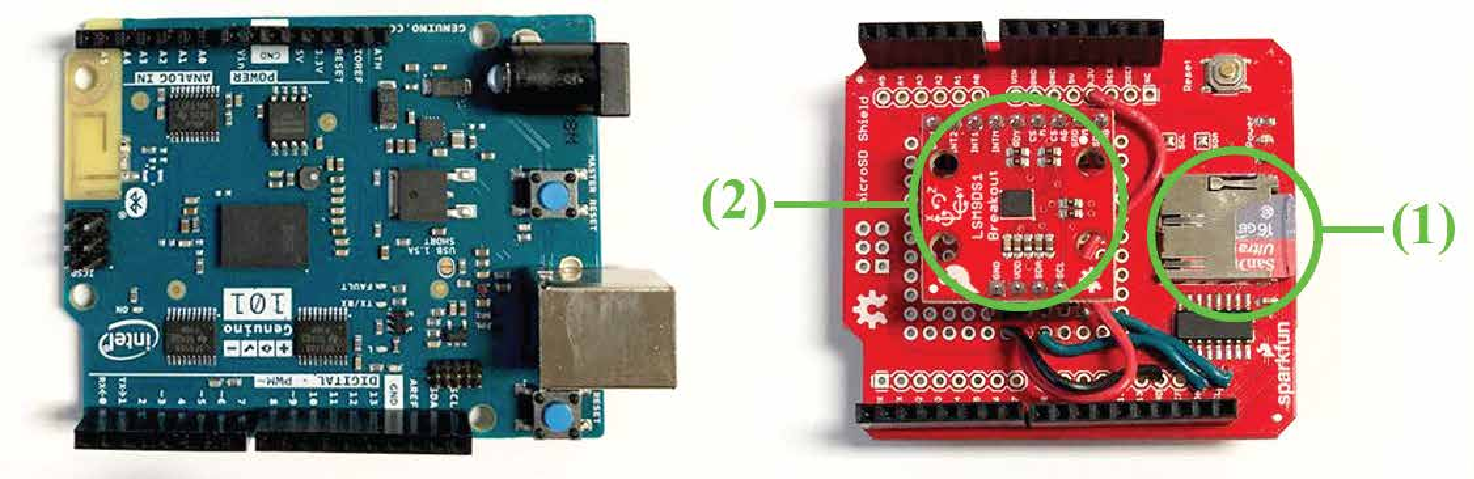
\includegraphics[width=.8\linewidth]{chapter4/device.pdf}
        \caption{\acs{SOC} Arduino 101 et son \textit{shield} de prototypage incluant une carte mémoire (1) ainsi que la centrale inertielle \textit{LSM9DS1} (2) présente sur la version 2 du dispositif.}
	\label{fig:device}
\end{figure}

\subsection{Le \textit{firmware}}

% \citep{Thullier2019}

Pour assurer le bon fonctionnement du matériel qui compose le \textit{wearable device} il était tout d'abord nécessaire de développer un \textit{firmware} \footnote{\url{https://github.com/FlorentinTh/SoilTypesRecognition-WearableFirmware}}. Le fonctionnement de celui-ci s'articule autour de trois composants logiciels principaux qui sont illustrés en figure \ref{fig:soil_types_firmware}.

\begin{figure}[H]
	\centering
	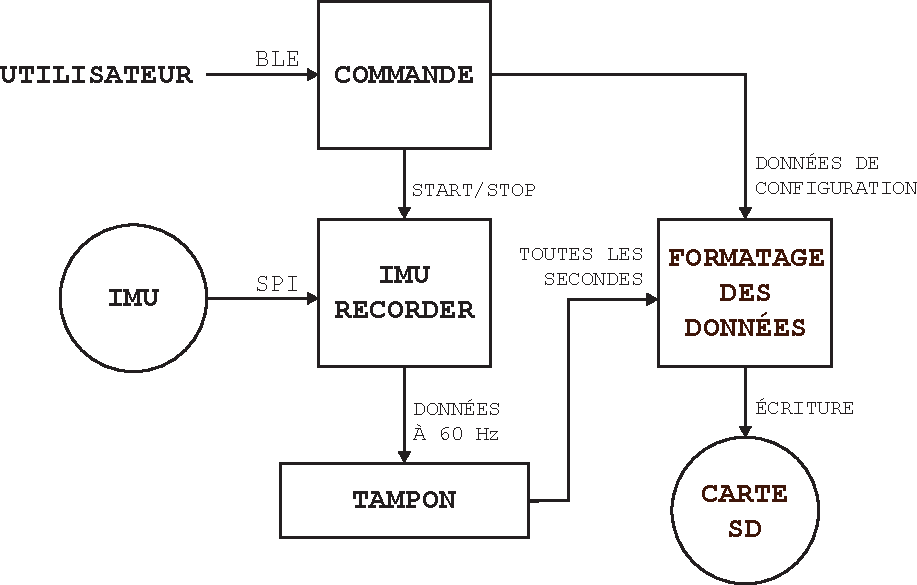
\includegraphics[width=12cm]{chapter4/soil_types_firmware.pdf}
        \caption{Représentation graphique de l'implémentation du \textit{firmware} embarqué sur le \textit{wearable device}.}
	\label{fig:soil_types_firmware}
\end{figure}

Le premier est le module de commande. Il est en charge des communications entre le téléphone et le dispositif par l'intermédiaire du module radio \acs{BLE}. Ainsi, un téléphone ou n'importe quel autre dispositif compatible avec la technologie \acs{BLE} peut être utilisé pour étiqueter les ensembles de données enregistrés avec les informations de configuration requises (le type de sol, l'identifiant anonyme du participant et l'emplacement du dispositif).

Le second module principal est l'\textit{\acs{IMU} Recorder}. En fonction de la version du dispositif, il a pour rôle de stocker dans une mémoire tampon les valeurs de l'\acs{IMU} qui transitent soit par un bus de données \ac{SPI} dans sa première version, soit \textit{via} un bus de données \ac{I2C}, à une fréquence stabilisée à $60\: Hz$.

Le contenu de la mémoire tampon est ensuite envoyé au module de formatage des données toutes les secondes. Finalement, ce composant récupère l'ensemble des données de configuration du module de commande et s'occupe d'écrire les nouvelles données dans un fichier \ac{CSV} qui est stocké sur la carte mémoire. Dans la seconde version du \textit{wearable device}, le module de formatage des données s'occupe également de calculer les angles d'Euler (précession, nutation et rotation propre) grâce aux trois axes supplémentaires fournis par le \textit{LSM9DS1}.

\subsection{Le processus d'apprentissage pour la reconnaissance des types de sols}

\subsubsection{Extraction des caractéristiques}

Après que les données aient été enregistrées sur la carte mémoire, le processus d'apprentissage pour la reconnaissance des types de sol est réalisé. Celui-ci débute par l'extraction des caractéristiques. En ce sens, cette solution propose d'utiliser les caractéristiques temporelles et fréquentielles les plus employées dans le domaine de la reconnaissance d'activités tel que discuté à la section \ref{sec:prel_steps} et qui sont rappelées par le tableau \ref{tab:features}.

\begin{table}[H]
	\caption{Récapitulatif de toutes les caractéristiques utilisées par la solution proposée en fonction du nombre d'axes offerts par la centrale inertielle.}
	\label{tab:features}
	\resizebox{\textwidth}{!}{%
	\begin{tabular}{|r|c|c|c|c|c|c|c|}
	\hline
	\multicolumn{4}{|c|}{\textbf{Domaine Temporel}} & \multicolumn{4}{c|}{\textbf{Domaine Fréquentiel}} \\ \hline
	\multicolumn{1}{|c|}{\multirow{3}{*}{\textit{\textbf{Caractéristique}}}} & \multicolumn{3}{c|}{\textit{\textbf{\begin{tabular}[c]{@{}c@{}}Nb. Total de\\[-15pt] Caractéristiques\end{tabular}}}} & \multirow{3}{*}{\textit{\textbf{Caractéristique}}} & \multicolumn{3}{c|}{\textit{\textbf{\begin{tabular}[c]{@{}c@{}}Nb. Total de\\[-15pt] Caractéristiques\end{tabular}}}} \\ \cline{2-4} \cline{6-8}
	\multicolumn{1}{|c|}{} & \textit{\begin{tabular}[c]{@{}c@{}}IMU \\[-15pt] 6 axes\end{tabular}} & \textit{\begin{tabular}[c]{@{}c@{}}IMU \\[-15pt] 9 axes\end{tabular}} & \textit{\begin{tabular}[c]{@{}c@{}}IMU \\[-15pt] 9 axes\\[-15pt] avec angles\\[-15pt] d'Euler\end{tabular}} &  & \textit{\begin{tabular}[c]{@{}c@{}}IMU \\[-15pt] 6 axes\end{tabular}} & \textit{\begin{tabular}[c]{@{}c@{}}IMU \\[-15pt] 9 axes\end{tabular}} & \textit{\begin{tabular}[c]{@{}c@{}}IMU \\[-15pt] 9 axes\\[-15pt] avec angles\\[-15pt] d'Euler\end{tabular}} \\ \hline
	Moyenne pour chaque axe & 6 & 9 & 12 & \multicolumn{1}{r|}{Composante continue pour chaque axe} & 6 & 9 & 12 \\ \hline
	Moyenne de tous les axes & 2 & 3 & 4 & \multicolumn{1}{r|}{\begin{tabular}[c]{@{}r@{}}Énergie spectrale pour chaque axe\\[-15pt] (équation \ref{eq:energy_spec})\end{tabular}} & 6 & 9 & 12 \\ \hline
	Écart type pour chaque axe & 6 & 9 & 12 & \multicolumn{1}{r|}{\begin{tabular}[c]{@{}r@{}}Entropie pour chaque axe\\[-15pt] (équation \ref{eq:entropy})\end{tabular}} & 6 & 9 & 12 \\ \hline
	Écart type pour tous les axes & 2 & 3 & 4 & - & - & - & - \\ \hline
	\begin{tabular}[c]{@{}r@{}}Asymétrie pour chaque axe\\[-15pt] (équation \ref{eq:asymetrie})\end{tabular} & 6 & 9 & 12 & - & - & - & - \\ \hline
	Asymétrie pour tous les axes & 2 & 3 & 4 & - & - & - & - \\ \hline
	\begin{tabular}[c]{@{}r@{}}Kurtosis pour chaque axe\\[-15pt] (équation \ref{eq:kurtosis})\end{tabular} & 6 & 9 & 12 & - & - & - & - \\ \hline
	Kurtosis pour tous les axes & 2 & 3 & 4 & - & - & - & - \\ \hline
	\begin{tabular}[c]{@{}r@{}}Corrélation entre toutes les combinaisons \\[-15pt] possibles d'axes incluant le total des axes\end{tabular} & 12 & 18 & 24 & - & - & - & - \\ \hline
	Zero Crossing Rate pour chaque axe & 6 & 9 & 12 & - & - & - & - \\ \hline
	Zero Crossing Rate pour tous les axes & 2 & 3 & 4 & - & - & - & - \\ \hline
	\textit{\textbf{Sous-total}} & \textit{\textbf{52}} & \textit{\textbf{78}} & \textit{\textbf{104}} & \multicolumn{1}{r|}{\textit{\textbf{Sous-total}}} & \textit{\textbf{18}} & \textit{\textbf{27}} & \textit{\textbf{36}} \\ \hline
	\multirow{4}{*}{\textbf{Total}} & \multicolumn{1}{r|}{\textit{\textbf{\begin{tabular}[c]{@{}r@{}}IMU\\[-15pt] 6 axes\end{tabular}}}} & \multicolumn{6}{c|}{\textbf{70}} \\ \cline{2-8}
	 & \multicolumn{1}{r|}{\textbf{\begin{tabular}[c]{@{}r@{}}IMU\\[-15pt] 9 axes\end{tabular}}} & \multicolumn{6}{c|}{\textbf{105}} \\ \cline{2-8}
	 & \multicolumn{1}{r|}{\textbf{\begin{tabular}[c]{@{}r@{}}IMU 9 axes\\[-15pt] avec angles d'Euler\end{tabular}}} & \multicolumn{6}{c|}{\textbf{140}} \\ \hline
	\end{tabular}%
	}
\end{table}

\noindent La première opération consiste en une simple moyenne non pondérée sur chacun des axes tant \og{}physiques\fg{} des capteurs de l'\acs{IMU} (gyroscope, accéléromètre et magnétomètre si 9-\acs{DOF}) que \og{}logiques\fg{} (angles d'Euler), s'ils existent. Ensuite, la moyenne générale de chacune de ces caractéristiques est calculée pour l'ensemble des axes. De la même manière, cette procédure a été appliquée à plusieurs autres calculs statistiques : l'écart type, l'asymétrie (équation \ref{eq:asymetrie}), le kurtosis (équation \ref{eq:kurtosis}), le \textit{Zero Crossing Rate} et la corrélation entre toutes les combinaisons possibles d'axes par capteurs de l'\acs{IMU} (équation \ref{eq:correlation}). Dans un second temps, une transformation du domaine temporel vers le domaine fréquentiel a été nécessaire pour obtenir les caractéristiques suivantes : la composante continue, l'énergie spectrale (équation \ref{eq:energy_spec}) et l'entropie  (équation \ref{eq:entropy}). Ce passage d'un domaine à l'autre a été réalisée en utilisant l'algorithme de la transformation de Fourier rapide (\acs{FFT}). Ainsi, en fonction de la centrale inertielle exploitée (6-\acs{DOF}, 9-\acs{DOF} ou 9-\acs{DOF} avec angles d'Euler), ce sont 70, 105 ou 140 caractéristiques qui sont calculées sur chaque fenêtre temporelle non chevauchante dont la taille est fixée à 60 secondes. La taille de la fenêtre a été déterminée par une évaluation du temps moyen nécessaire pour marcher une distance de $4.3\: m$, ce qui correspond à un aller-retour dans le bac utilisé lors des expérimentations et dont le protocole est décrit à la section \ref{sec:expe}.

\subsubsection{Apprentissage}

Dès l'obtention des caractéristiques discriminantes, l'étape suivante requise pour réaliser la reconnaissance des sols est le processus d'apprentissage. Selon la littérature qui concerne la reconnaissance d'activités, mais également celle au sujet de la reconnaissance des sols en robotique discutée dans les sections \ref{sec:algos} et \ref{sec:t1-related-work}, la performance de plusieurs algorithmes d'apprentissage a été démontrée. Néanmoins, ce premier travail propose une comparaison entre deux algorithmes qui n'ont pas encore été présentés dans cette thèse : la forêt d'arbres décisionnels et les $k$ plus proches voisins (\acl{KNN} ou \acs{KNN}). Ce choix est motivé par deux raisons principales. La première est que ces deux techniques d'apprentissage appartiennent à deux familles distinctes\textemdash respectivement, les arbres de décision et les algorithmes d'apprentissage \og{}paresseux\fg{}. De plus, ceux-ci constituent tous deux des méthodes non paramétriques, c'est-à-dire, qui ne font aucune supposition quant à la distribution de l'échantillon de données fournies en entrée. De ce fait, ces méthodes demeurent simples, flexibles puissants et efficaces \citep{Russell2010}. Par ailleurs, la performance en termes de taux de reconnaissance obtenue avec ces algorithmes est souvent exposée dans la littérature \citep{Kertesz2016, Vail2004}.

Selon \cite{Breiman2001}, une forêt d'arbres décisionnels est une combinaison d'arbres prédicteurs, aussi appelés arbre de décision, où chacun d'eux dépend d'un vecteur de données distinct, mais de même cardinalité. Ce vecteur contient un sous-ensemble aléatoire des données initiales issues de la phase d'extraction des caractéristiques. La décision finale du processus de reconnaissance de cet algorithme est déterminée par un vote majoritaire entre chacune des décisions émises en sortie des arbres de décision qui composent la forêt. La figure \ref{fig:algo_random_forest} illustre un exemple simplifié d'une forêt d'arbres décisionnels utilisant trois arbres.

\begin{figure}[H]
	\centering
	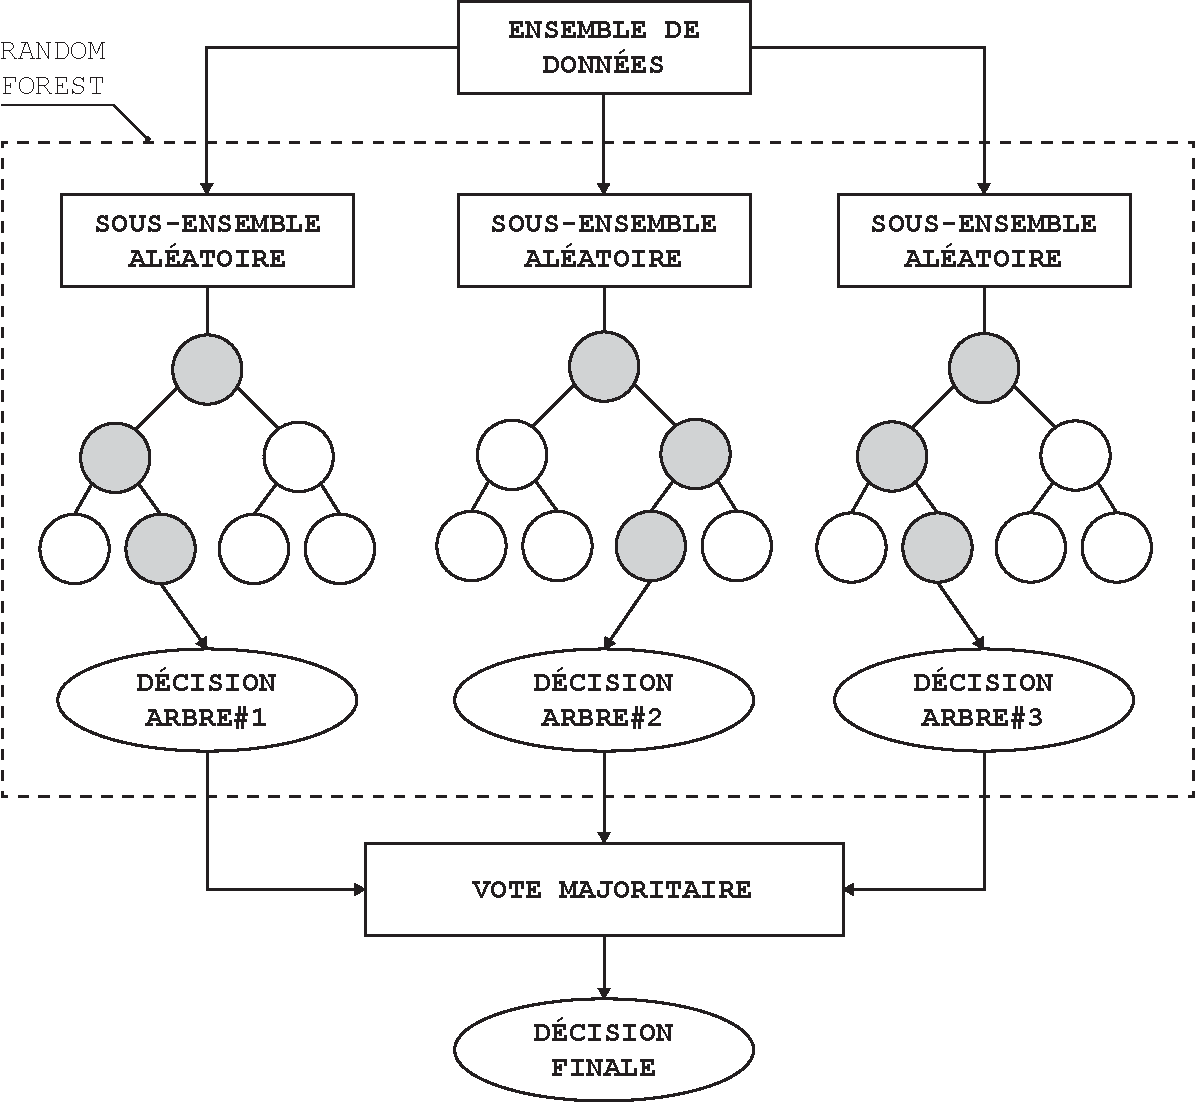
\includegraphics[width=12cm]{chapter4/algo_random_forest.pdf}
        \caption{Exemple de l'algorithme \textit{Random Forest} utilisant $B=3$ arbres.}
	\label{fig:algo_random_forest}
\end{figure}

Pour exploiter la forêt d'arbres décisionnels en tant qu'algorithme d'apprentissage, il est important de définir préalablement au moins trois paramètres principaux. Le premier est le nombre d'arbres que doit comporter la forêt ($B$). Le second correspond au nombre de caractéristiques à considérer dans la division des n\oe{}uds de l'arbre lors de la construction de ce dernier ($F$) et enfin, la fonction nécessaire à la mesure de la qualité de cette division ($C$). En ce qui concerne le nombre de caractéristiques, \citeauthor{Breiman2001} suggère d'utiliser $F=log_2(m) + 1$ ou $m$ fait référence au nombre total d'attributs présents dans le jeu de données fourni en entrée. Néanmoins, il est également possible de trouver d'autres recommandations comme $F=\frac{1}{2}\sqrt{m}$ ou encore $F=\sqrt{m}$. Par ailleurs, en ce qui concerne la mesure de la qualité de la division des n\oe{}uds les fonctions qui sont les plus couramment utilisées sont le calcul du c\oe{}fficient de Gini et l'évaluation du gain en information basé sur l'entropie de Shannon dont les équations sont respectivement rappelées ci-après :

\begin{equation}
	\label{eq:gini}
	C(T) = Gini(T) = {1-\sum_{i=1}^{n}(p_i)}^2
\end{equation}

\begin{equation}
	\label{eq:gain}
	C(T) = E(T) = \sum_{i=1}^{n}-(p_i log_2 p_i)
\end{equation}

\noindent où $T$ correspond aux données qui contiennent les instances de $n$ étiquettes et $p_i$ est la fréquence relative de l'étiquette $i \in n$ dans $T$. Le choix quant à ce paramètre dépend essentiellement du type d'arbres de décision qui sont utilisés lors de la construction de la forêt (\textit{p. ex.} ID3, $C4.5$, CART, \textit{etc.}).

D'autre part, l'algorithme des $k$ plus proches voisins est considéré comme une technique d'apprentissage dite \og{}paresseuse\fg{} ce qui veut dire qu'il n'admet pas de phase d'entraînement, ou que celle-ci demeure minime. Bien que cet algorithme soit relativement rapide et flexible, la décision finale d'étiquetage est réalisée en se basant sur l'intégralité du jeu de données utilisé pour l'entraînement. En conséquence, celui-ci doit être stocké en mémoire, ce qui implique alors de disposer d'une quantité de stockage importante. En effet, cette méthode suppose que les données peuvent être représentées dans un espace vectoriel de caractéristiques qui peut être multidimensionnel. Ainsi, la phase d'apprentissage de l'algorithme consiste seulement à stocker ses vecteurs ainsi que les étiquettes qui leur sont associés. Ensuite, lors de la phase de reconnaissance il s'agit de déterminer quels sont les $k$ vecteurs de caractéristiques qui sont les plus proches pour chaque nouvelle donnée à étiqueter, où $k$ est un paramètre qui doit être défini antérieurement. Ces plus proches voisins sont alors extraits grâce à une fonction de mesure qui doit également être déterminée au préalable (\textit{p. ex.} la distance Euclidienne ou la distance de Manhattan respectivement données en équations \ref{eq:dist_euclidean} et \ref{eq:dist_manhattan}). Finalement, l'étiquette de la nouvelle donnée est alors attribuée selon un vote majoritaire entre celles de chaque $k$ plus proche voisin. La figure \ref{fig:algo_knn} illustre un exemple de cette méthode d'apprentissage lorsque $k=3$ plus proches voisins.

\begin{figure}[H]
	\centering
	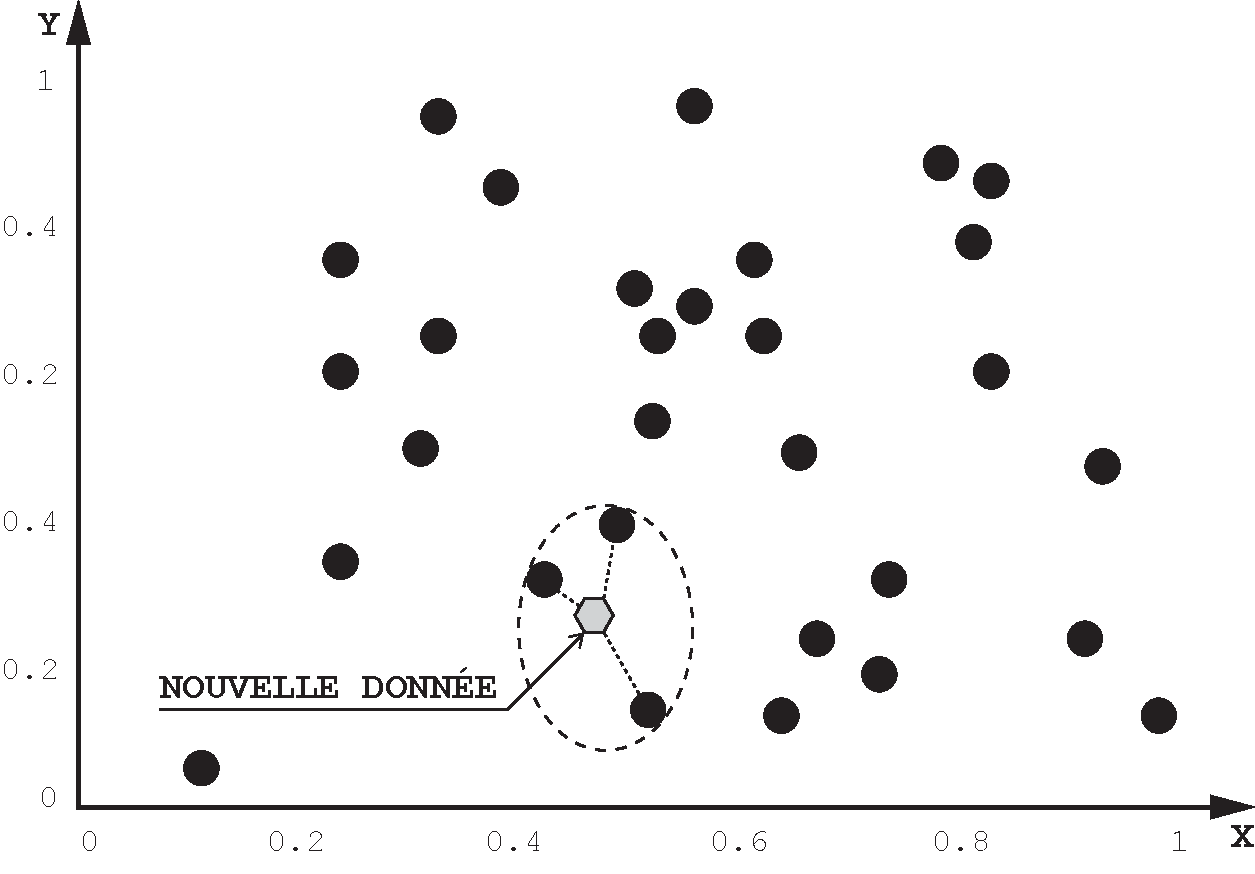
\includegraphics[width=10cm]{chapter4/algo_knn.pdf}
        \caption{Exemple de l'algoritme des $k$ plus proches voisins où $k=3$.}
	\label{fig:algo_knn}
\end{figure}

\section{Expérimentations}
\label{sec:expe}

Les expérimentations mises en place pour valider le système de reconnaissance des sols se sont déroulées en deux étapes et à deux périodes de l'année différentes. La première a été réalisée en hiver, avec la première version du \textit{wearable device} : $wear\_v1$. Elle a impliqué neuf étudiants universitaires, tous des hommes ayant entre 22 et 36 ans. Leurs poids se situaient entre $65\: kg$ et$ 110\: kg$ (poids médian : $80\: kg$) et leurs tailles étaient comprises entre $172\: cm$ et $192\: cm$ (taille médiane : $183\: cm$). Parmi ceux-ci, il y avait 7 droitiers pour 2 gauchers et tous étaient en bonne santé sans aucun problème de motricité. La seconde étape, quant à elle, s'est déroulée en été avec la deuxième version du dispositif : $wear\_v2$ et un téléphone intelligent : $cell$ (\textit{Huawei Nexus 6P} avec la version $8.0$ d'\textit{Android}). Cependant, seulement six participants sur les neuf de la première étape ont été en mesure de mener à bien cette seconde expérimentation.

\subsection{Mise en \oe{}uvre}

Dans un premier temps, puisque l'\acs{UQAC} se situe dans une région où les conditions météorologiques peuvent être difficiles, la plupart des différents types de sols sont, en fonction de la période de l'année, recouverts de glace ou de neige. Pour pallier cette problématique, un bac a été fabriqué afin d'assurer le déroulement des expérimentations à l'intérieur du laboratoire. Le contenu de celui-ci était soit du gravier soit du sable, tel qu'illustré par la figure \ref{fig:box}.

\begin{figure}[H]
	\centering
	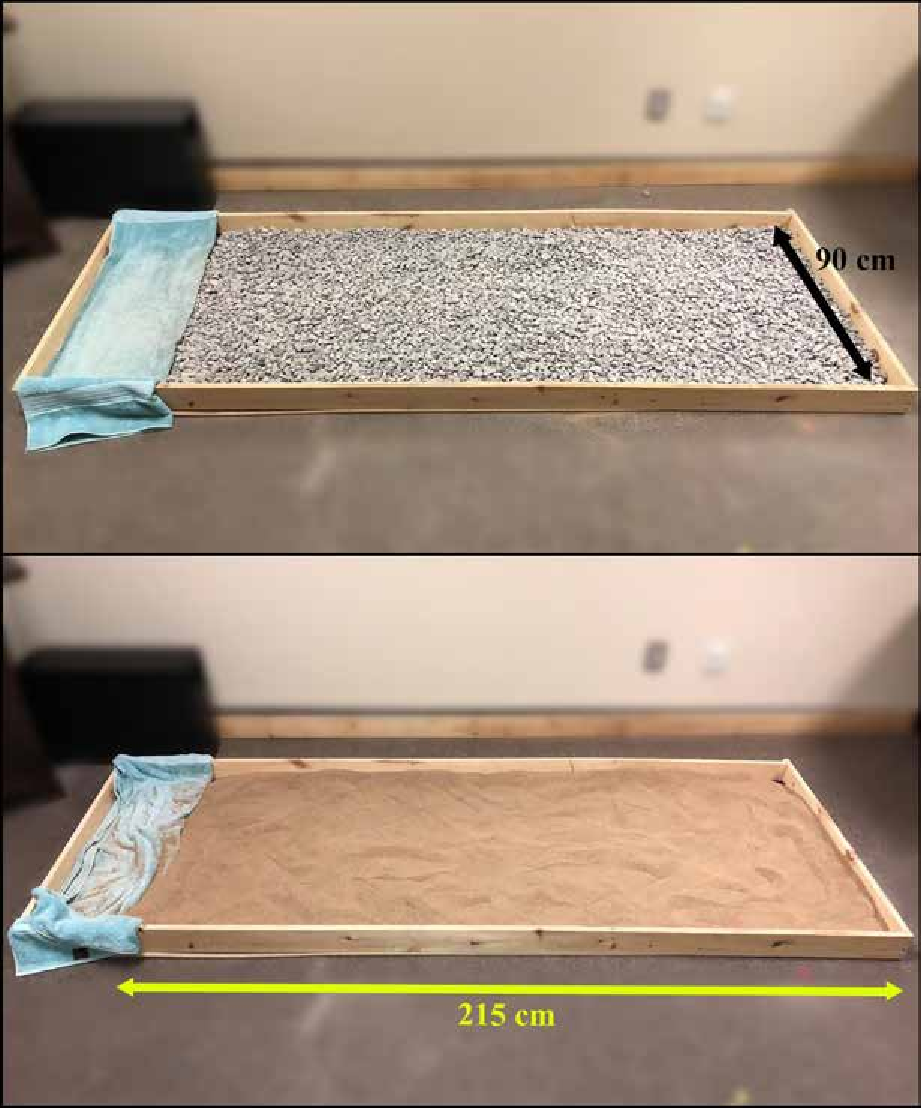
\includegraphics[width=.8\linewidth]{chapter4/box.pdf}
        \caption{Bac utilisé lors des expérimentations rempli de gravier en haut et de sable en bas, de dimensions: $l : 215\; cm \times L : 90\; cm \times H : 15\; cm$.}
	\label{fig:box}
\end{figure}

Dans un deuxième temps, une application \textit{Android}\footnote{\url{https://github.com/FlorentinTh/SoilTypesRecognition-AndroidAppDriver}} a été développée afin de piloter les expérimentations et par conséquent, annoter les jeux de données pour chacun des enregistrements produits par les participants. Ainsi, cette dernière a permis de définir les temps de début et de fin, ainsi que les différentes informations de configuration (le type de sol, l'identifiant anonyme du participant et l'emplacement du dispositif) par le biais d'un téléphone intelligent spécifiquement dédié à cette tâche : $cell\_oper$ (\textit{LG Nexus 5} avec la version $6.0.1$ d'\textit{Android}). Puisque le \textit{wearable device} est doté d'une connectivité \acs{BLE}, la première opération consiste à réaliser un balayage afin d'obtenir la liste des appareils dont le \acs{BLE} est actif aux alentours. Dans notre cas, $cell\_oper$ est le dispositif périphérique et le \textit{wearable device} est le dispositif central. Ensuite, dès que les deux appareils sont couplés, le \textit{wearable device} devient alors le serveur \acs{GATT} et $cell\_oper$ le client, tel qu'illustré par le premier ecran de la figure \ref{fig:application}. Enfin, l'enregistrement des données sur le \textit{wearable device} débute dès lors que les informations de configuration sont renseignées et que le bouton d'envoi des données est appuyé, comme le montre le second écran de la figure \ref{fig:application}

\begin{figure}[H]
	\centering
	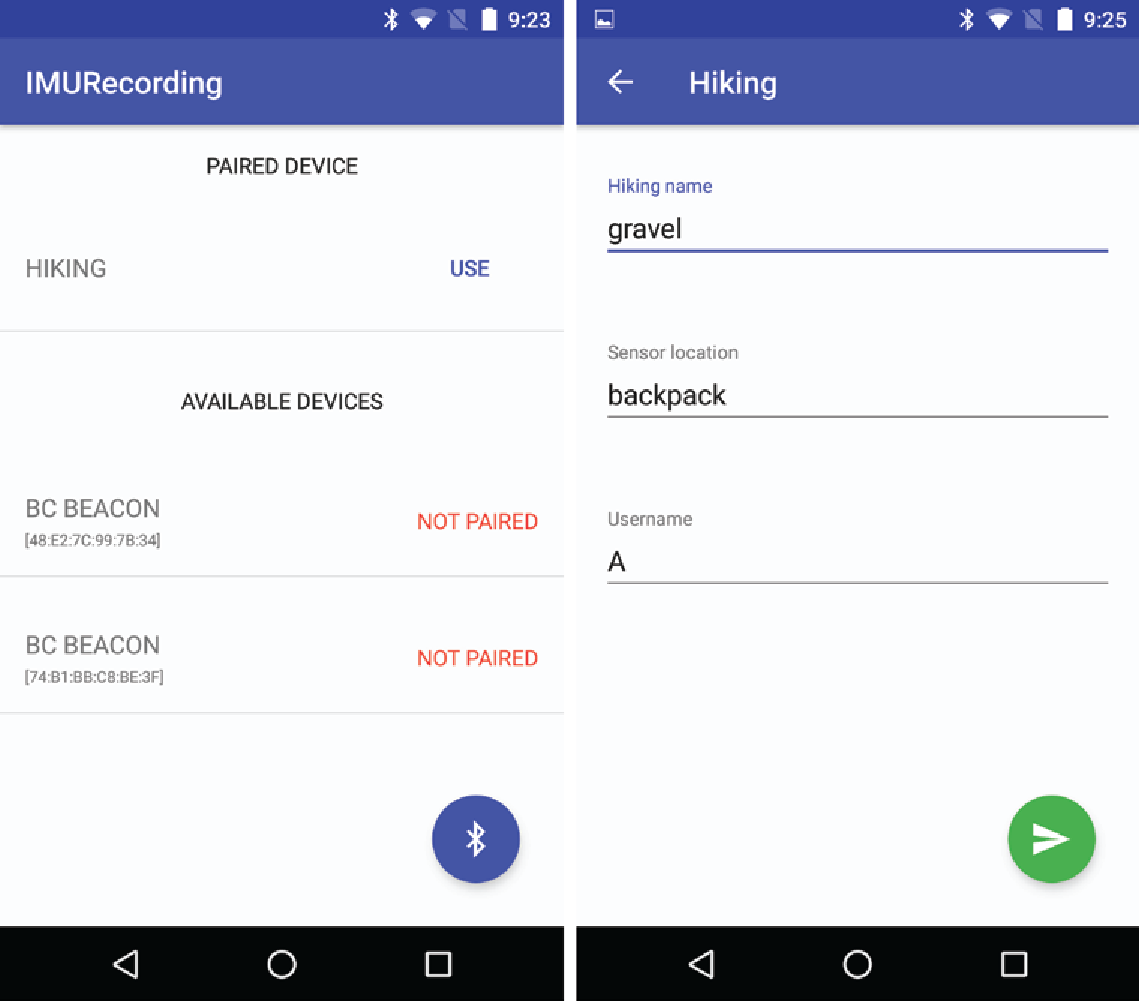
\includegraphics[width=.8\linewidth]{chapter4/application.pdf}
        \caption{Captures d'écran de l'application \textit{Android} qui permet de piloter et d'étiquetter les données enregistrées exécutée sur $cell\_oper$}
	\label{fig:application}
\end{figure}

\noindent L'avantage principal de cette méthode réside princiapelement dans la mobilité qu'offre l'utilisation d'un téléphone intelligent par rapport à un ordinateur traditionnel\textemdash ce qui a fortement facilité la tâche de supervision des expérimentations. De plus, l'application a pu être réutilisée sans subir de modifications aussi bien avec les deux versions du \textit{wearable device} ($wear\_v1$ et $wear\_v2$) qu'avec le téléphone intelligent utilisé pour l'enregistrement de données ($cell$).

Par ailleurs, le fonctionnement de la seconde application \textit{Android}\footnote{\url{https://github.com/FlorentinTh/SoilTypesRecognition-AndroidAppRecording}} qui a été développée demeure identique à celui du firmware du \textit{wearable device}. En effet, celle-ci reçoit par \acs{BLE} les mêmes informations de configuration envoyées par le biais de l'application qui s'exécute sur $cell\_oper$. De la même manière, les données inertielles (accéléromètre, gyroscope, magnétomètre) ainsi que les angles d'Euler sont enregistrés toutes les secondes sur la mémoire flash du téléphone sur lequel elle est exécutée ($cell$) au format \acs{CSV} à une même fréquence stabilisée à $60\: Hz$.

\subsection{Procédure}


\begin{figure}[H]
    \centering
	\subfloat[De gauche à droite, positionnement du \textit{wearable device} dans les poches de droite (1) et de gauche (2) ainsi qu'à l'intérieur d'un sac à dos ordinaire de 20L.]{
		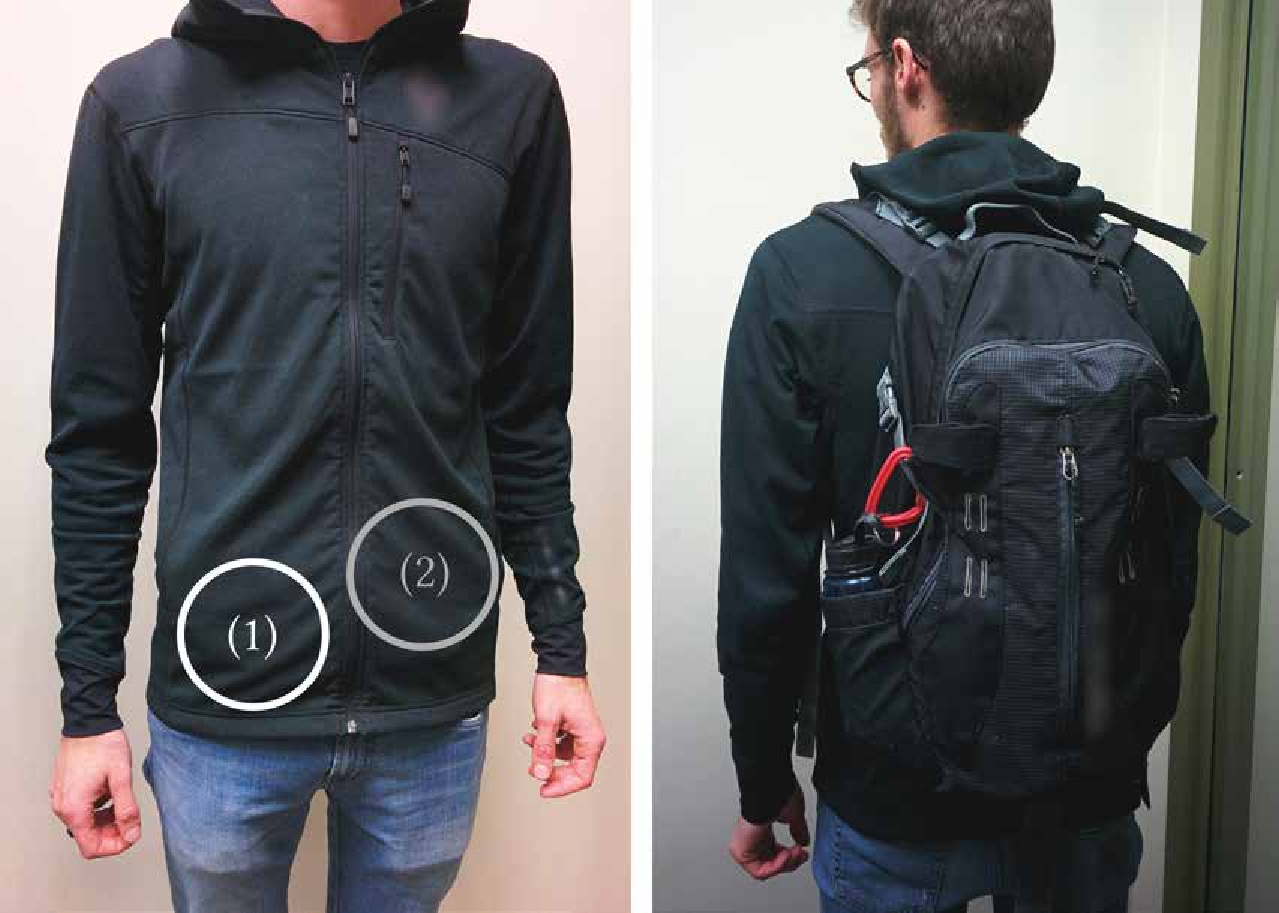
\includegraphics[width=.7\linewidth]{chapter4/positions_a.pdf}
		\label{fig:positions_a}
    }
    \\[30pt]
	\subfloat[Positionnement du \textit{wearable device} à l'intérieur d'un sac bandoulière porté sur les épaules de droite et de gauche.]{
		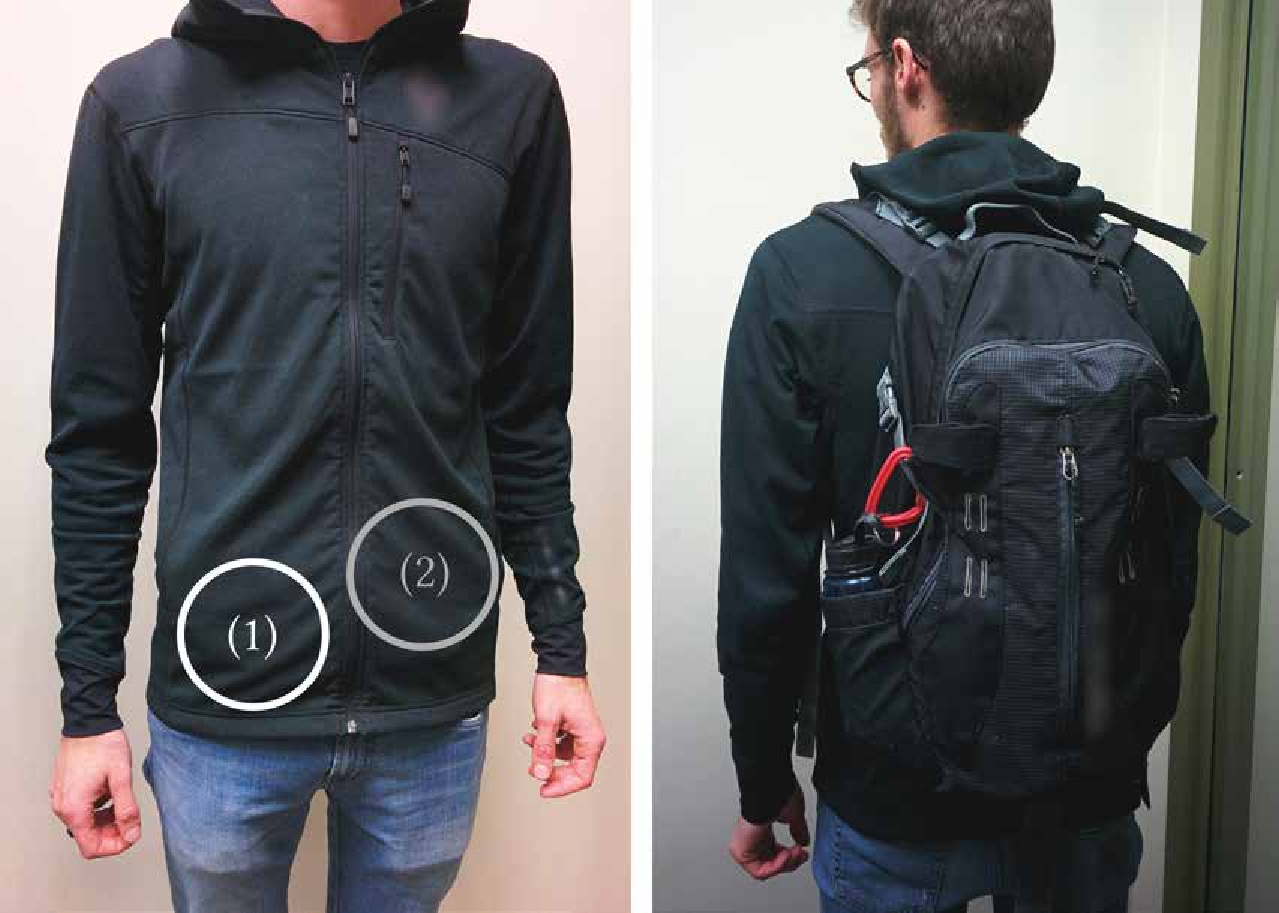
\includegraphics[width=.7\linewidth]{chapter4/positions_b.pdf}
		\label{fig:positions_b}
    }
    \caption{Illustration des cinq emplacements où le \textit{wearable device} est positionné pendant l'expérimentation.}
    \label{fig:positions}
\end{figure}

\section{Résultats et discussion}

\subsection{Ensembles de données}

\begin{table}[H]\renewcommand{\arraystretch}{0.5}
	\begin{center}
		\caption{Liste des datasets.}
		\label{tab:datasets}
		\begin{tabular}{@{}rl@{}}
			\toprule
				\textbf{Dataset} & \textbf{Description} \\
			\midrule
				\textbf{soil\_type\_{[}\textit{wear\_v1}|\textit{wear\_v2}|\textit{cell}{]}\_{[}\textit{6}|\textit{9}|\textit{12}{]}} & Lorem \\
				\textbf{soil\_type\_position\_{[}\textit{wear\_v1}|\textit{wear\_v2}|\textit{cell}{]}\_{[}\textit{6}|\textit{9}|\textit{12}{]}} & Lorem \\
			\bottomrule
		\end{tabular}
	\end{center}
\end{table}

\subsection{Résultats obtenus}

\subsubsection{\textit{Version 1 du wearable device}}

\begin{figure}[H]
    \centering
	\subfloat[RF]{
		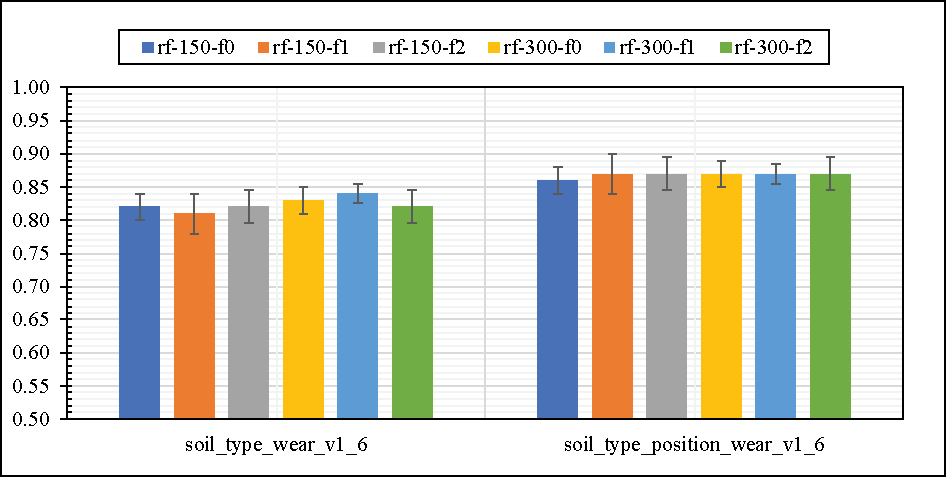
\includegraphics[width=.8\linewidth]{chapter4/results_wear_v1_rf.pdf}
		\label{fig:results_wear_v1_rf}
    }
    \\[20pt]
	\subfloat[KNN]{
		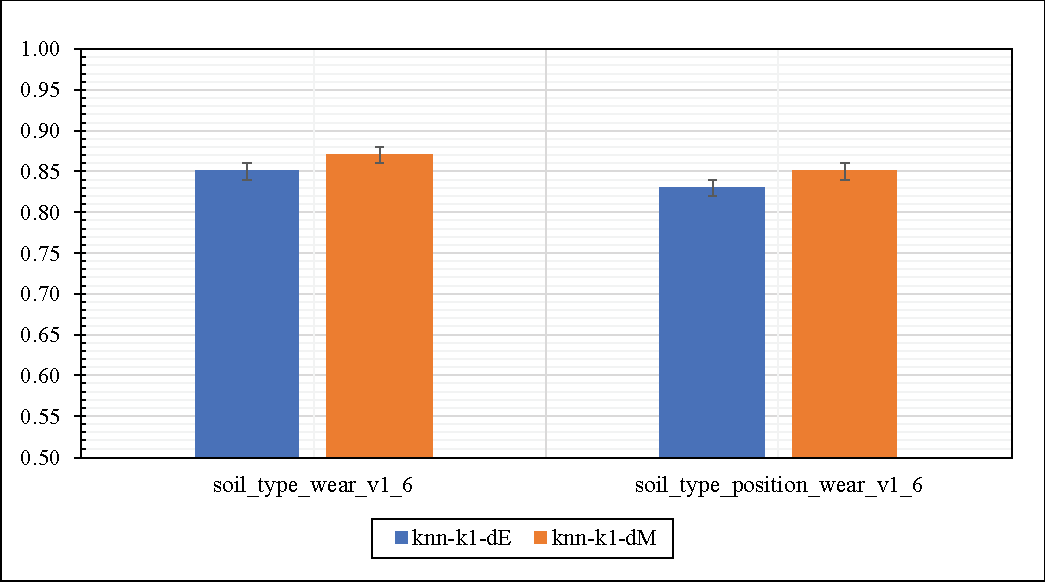
\includegraphics[width=.8\linewidth]{chapter4/results_wear_v1_knn.pdf}
		\label{fig:results_wear_v1_knn}
    }
    \caption{Résultats.}
    \label{fig:results_wear_v1}
\end{figure}

\begin{figure}[H]
    \centering
	\subfloat[RF]{
		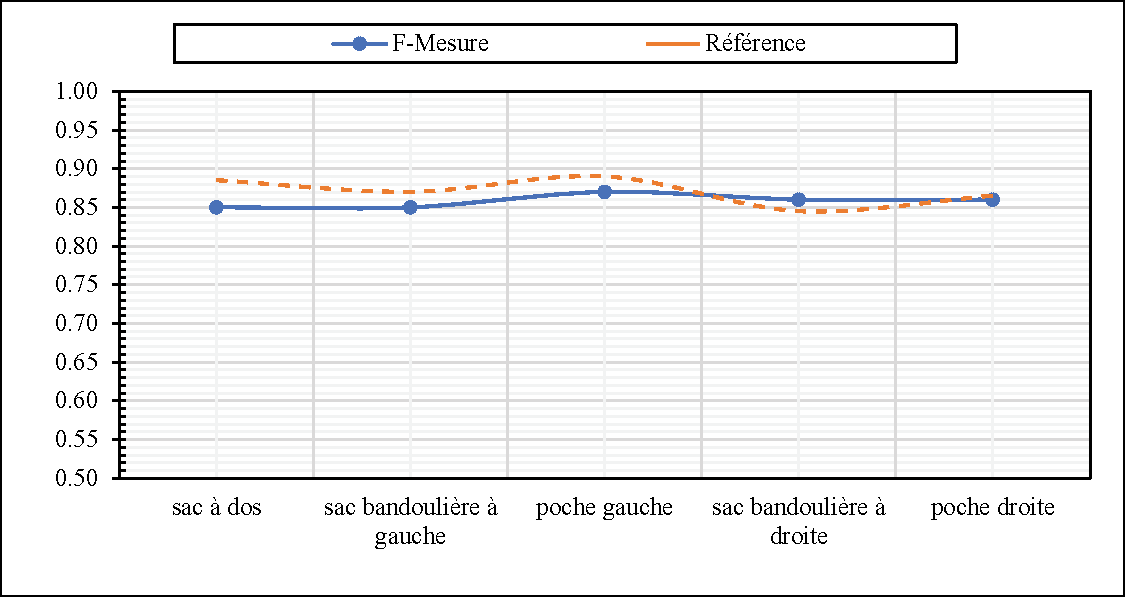
\includegraphics[width=.8\linewidth]{chapter4/pos_ind_rf_wear_1.pdf}
		\label{fig:pos_ind_rf_wear_1}
    }
    \\[20pt]
	\subfloat[KNN]{
		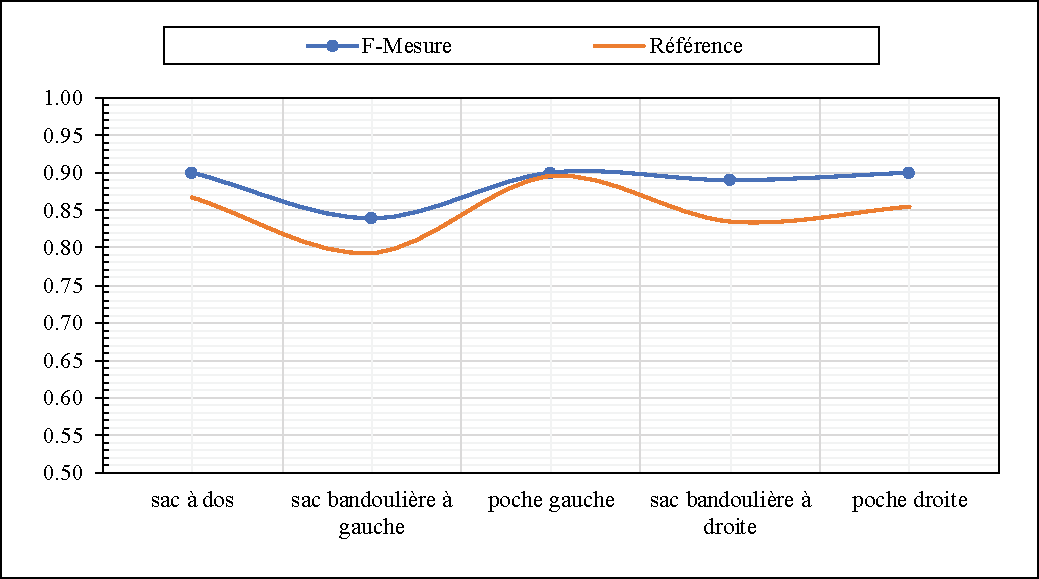
\includegraphics[width=.8\linewidth]{chapter4/pos_ind_knn_wear_1.pdf}
		\label{fig:pos_ind_knn_wear_1}
    }
    \caption{Indépendance de posisition.}
    \label{fig:pos_ind_wear_v1}
\end{figure}

\subsubsection{\textit{Version 2 du wearable device}}

\begin{figure}[H]
	\centering
	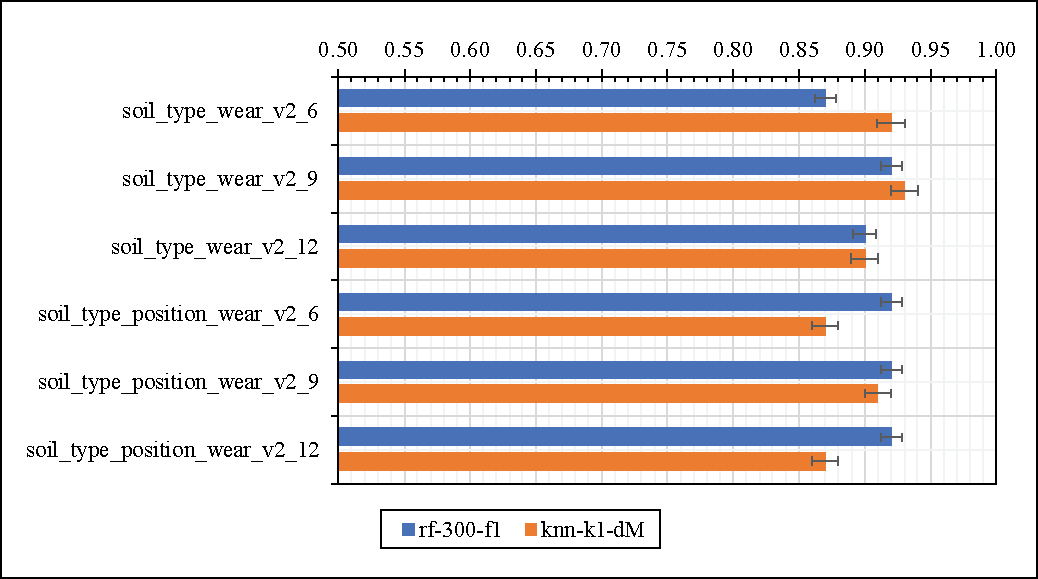
\includegraphics[width=.8\linewidth]{chapter4/results_wear_v2.pdf}
        \caption{Résultats.}
	\label{fig:results_wear_v2}
\end{figure}

\begin{figure}[H]
    \centering
	\subfloat[RF]{
		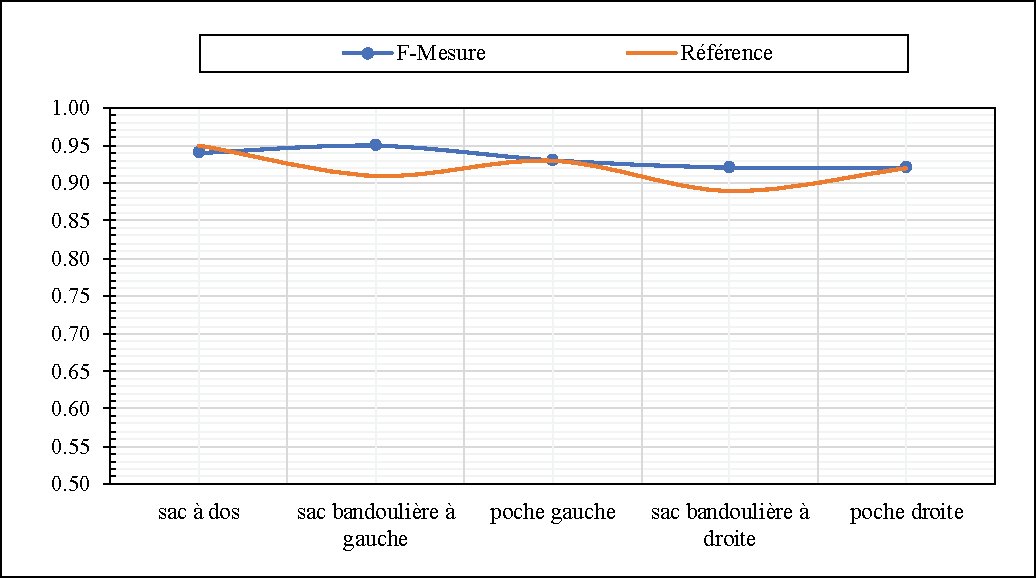
\includegraphics[width=.8\linewidth]{chapter4/pos_ind_rf_wear_2.pdf}
		\label{fig:pos_ind_rf_wear_2}
    }
    \\[20pt]
	\subfloat[KNN]{
		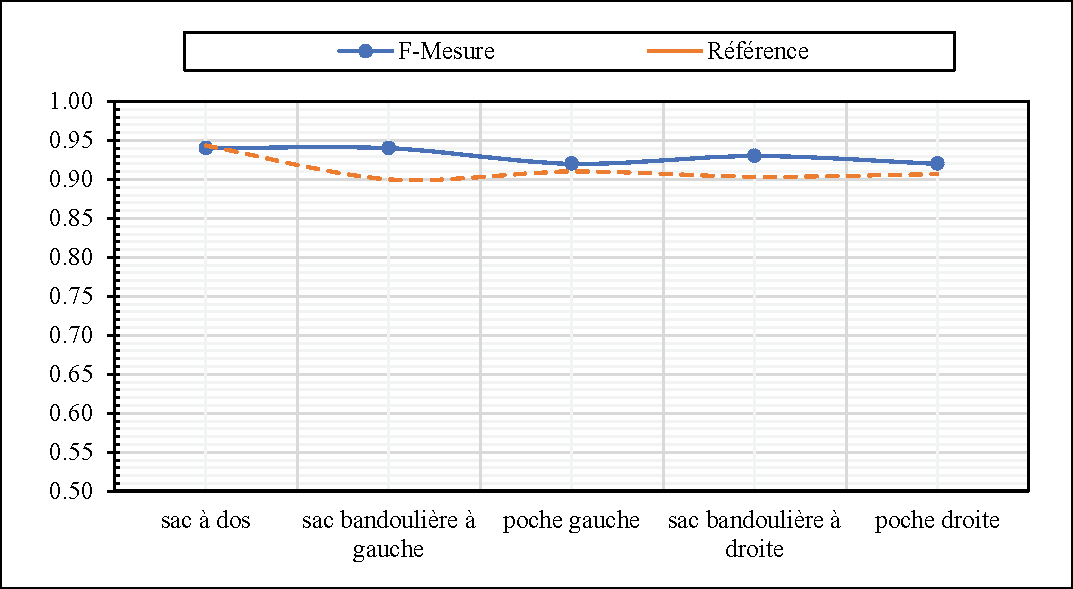
\includegraphics[width=.8\linewidth]{chapter4/pos_ind_knn_wear_2.pdf}
		\label{fig:pos_ind_knn_wear_2}
    }
    \caption{Indépendance de posisition.}
    \label{fig:pos_ind_wear_v2}
\end{figure}

\subsubsection{\textit{Téléphone intelligent}}

\begin{figure}[H]
	\centering
	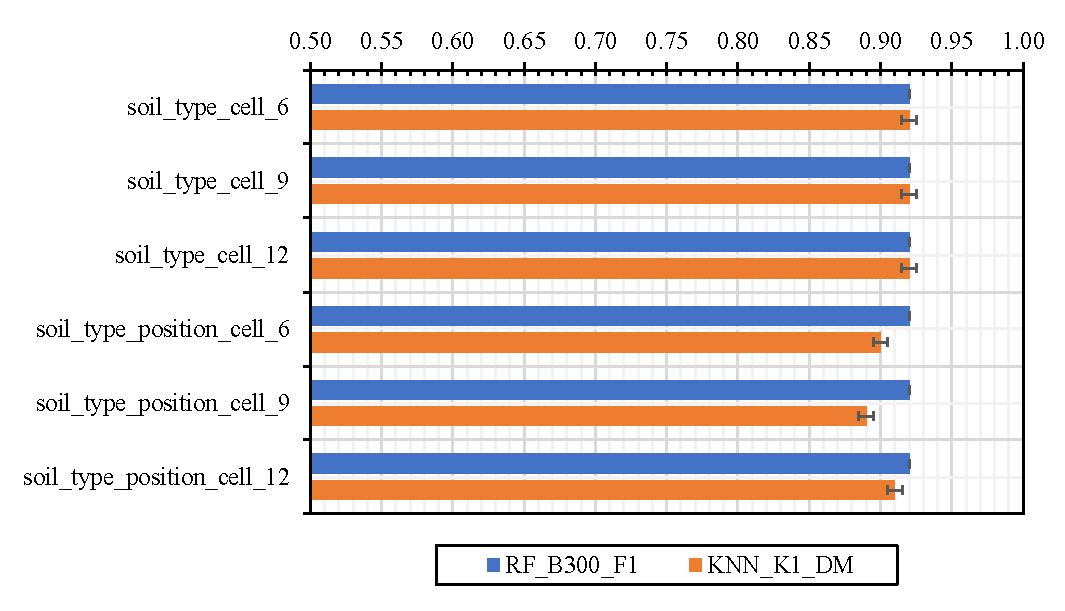
\includegraphics[width=.8\linewidth]{chapter4/results_cell.pdf}
        \caption{Résultats.}
	\label{fig:results_cell}
\end{figure}

\subsection{Discussion des résultats obtenus}

\section{Conclusion}